\documentclass[a4paper, adobefonts]{ctexart}

\usepackage[top=1.2in, bottom=1.2in, left=1in, right=1in]{geometry}
\usepackage{minted, graphicx, hyperref}

\hypersetup{colorlinks=true, linkcolor=blue}

\title{操作系统实验报告6}
\author{蔡日骏\quad12348003}

\begin{document}
\maketitle
\tableofcontents

\section{概述}
本实验中实现了一个保护模式多任务分页内核AssignmentOS。其中多任务使用x86硬件多任务
实现。由于文件系统部分尚未实现,目前用户程序只能与内核一同编译。另外,由于中断驱动
程序尚未实现双缓冲输出,因此在用户态尚未支持多屏、分屏显示。目前版本只能作多任务
演示,完整功能的内核将在以后版本中实现。

\section{构建指南}
AssignmentOS编译需要一个默认目标为~\verb|i386-elf|的GCC、GNU Make、gzip。
安装时则需要dd、mount/pmount等程序进行软盘镜像操作。此外,AssignmentOS还需要GRUB Legacy
或GRUB 2等支持Multiboot标准的引导器进行启动。

\subsection{编译}
由于已有~\verb|Makefile|,因此可以直接运行~\verb|make|命令进行编译。但是为了让~\verb|make|
能够找到需要的构建工具链,一般需要先进行环境变量设置。可以设置的环境变量有两个,
一个是~\verb|CC|,用于指定需要使用的C编译器(目前仅在默认目标为~\verb|i386-elf|的
GCC 4.8.2上进行过测试);另一个是~\verb|EXTRAFLAGS|,用于指定额外的编译参数(默认
为空,可以使用~\verb|-O2|打开编译优化,\verb|-g|添加调试信息)。

编译完成后会自动进行内核压缩。

\subsection{安装}
编译出来的内核需要安装在软盘上,由GRUB Legacy或GRUB 2引导。下面以FAT12格式软盘、
GRUB Legacy(0.97)为例。

\begin{enumerate}
    \item 准备FAT格式软盘镜像。

\begin{verbatim}
$ dd if=/dev/zero of=disk.img count=2880
$ mkfs -t fat -F 12 disk.img
\end{verbatim}

    \item 挂载软盘镜像,把AssignmentOS内核镜像和GRUB镜像文件复制进去,挂在软盘
        镜像可以使用直接使用~\verb|mount|程序,但是这样要处理权限问题。更简单的
        方法是使用用户态的挂载程序,下面以~\verb|pmount|为例。

\begin{verbatim}
$ pmount disk.img
$ mkdir -p /media/disk.img/boot/grub
$ cp kernel.gz /media/disk.img/boot
$ cp menu.lst /media/disk.img/boot/grub
$ cd /usr/lib/grub
$ cp stage1 fat_stage1_5 stage2 /media/disk.img/boot/grub
\end{verbatim}

        其中GRUB的配置文件~\verb|menu.lst|内容如下。

\begin{verbatim}
timeout 5
default 0
color light-blue/black light-cyan/blue

title AssignmentOS Version 1.0
root (fd0)
kernel /boot/kernel.gz
\end{verbatim}

    \item 安装GRUB。安装前需要使用~\verb|sync|命令刷新系统的IO缓冲区保证前面的文件
        正确写入软盘镜像。

\begin{verbatim}
$ sync
$ grub
\end{verbatim}

        在GRUB Shell中运行以下命令。

\begin{verbatim}
grub> device (fd0) disk.img
grub> root (fd0)
grub> setup (fd0)
\end{verbatim}

        随后刷新缓冲区即可。

\end{enumerate}

\section{内核架构}
下面对AssignmentOS内核的架构进行简单介绍。

\subsection{源文件目录}
\begin{verbatim}
.
|-- kernel
|   |-- boot
|   |   |-- boot.asm            内核头部
|   |   |-- Makefile
|   |-- drivers                 驱动程序目录
|   |   |-- keyboard_map.c      键盘映射信息
|   |   |-- Makefile
|   |   |-- tty.c               终端驱动程序
|   |-- include
|   |   |-- constants.h         常数定义
|   |   |-- interrupts.h        中断子系统头文件
|   |   |-- kernel.h            内核全局头文件
|   |   |-- keyboard.h          键盘驱动程序头文件
|   |   |-- keyboard_map.h      键盘映射信息头文件
|   |   |-- mm.h                内存管理子系统头文件
|   |   |-- scheduler.h         任务调度子系统头文件
|   |   |-- timer.h             定时器子系统头文件
|   |   |-- tty.h               终端驱动程序头文件
|   |   |-- utils.h             工具函数头文件
|   |-- interrupts
|   |   |-- idt.c               中断描述符表操作
|   |   |-- int_handlers.asm    中断处理函数包装
|   |   |-- keyboard.c          键盘驱动程序
|   |   |-- Makefile
|   |   |-- pic.c               可编程中断控制器操作
|   |   |-- timer.c             定时器子系统
|   |-- mm
|   |   |-- Makefile
|   |   |-- mm.c                内存管理子系统
|   |   |-- paging.c            分页控制
|   |-- scheduler
|   |   |-- Makefile
|   |   |-- scheduler.c         任务调度子系统
|   |-- utils
|   |   |-- Makefile
|   |   |-- utils.asm           工具函数
|   |-- link.ld                 内核链接脚本
|   |-- main.c                  内核主函数
|   |-- Makefile
|   |-- programs.c              演示用户程序
|   |-- shell.c                 Shell程序
|-- Makefile
\end{verbatim}

\subsection{基本架构}
AssignmentOS是一个保护模式的内核,使用分页机制进行内存管理,任务调度使用x86硬件
多任务方式进行上下文切换。内核格式为ELF32格式,根据Multiboot标准进行引导。

GRUB把AssignmentOS内核加载到内存~\verb|0x100000|起始的位置并跳转到~\verb|boot.asm|
中的内核入口点~\verb|_start|,\verb|boot.asm|进行全局描述符表的初始化后跳转到~\verb|main.c|
中的内核主函数~\verb|kmain|进行进一步的初始化。~\verb|kmain|完成内核初始化后会
加载Shell程序,等待调度器把控制权交给Shell程序,至此系统启动完成。

\verb|boot.asm|的文本段如下。

\begin{minted}{nasm}
section .text
global _start
_start:
    mov esp, stack_top      ;把ESP指向内核堆栈栈顶

    lgdt [gdtr]             ;加载全局描述符表

    mov ax, 2<<3            ;更新数据段寄存器
    mov ds, ax
    mov es, ax
    mov fs, ax
    mov gs, ax
    mov ss, ax

    jmp 0x8:after_lgdt      ;更新数据段寄存器
after_lgdt:

    push ebx                ;向内核主函数传递Multiboot数据
    extern kmain
    call kmain              ;调用内核主函数

.hang:
    hlt                     ;初始化完成后在这里挂起,等待调度器接管
    jmp .hang
\end{minted}

\verb|kmain|内核主函数如下。

\begin{minted}{c}
void kmain(void *mb_info)   /* mb_info为GRUB传递过来的Multiboot数据 */
{
    cli();                  /* 关闭中断 */
    init_variables();       /* 初始化某些内核全局变量 */
    enable_paging();        /* 启动内存分页 */
    init_mm(((uint32_t *)mb_info)[2]);  /* 初始化内存管理子系统 */
    init_idt();             /* 初始化中断描述符表 */
    init_pic();             /* 初始化可编程中断控制器 */
    init_timer();           /* 初始化定时器子系统 */
    init_kb();              /* 初始化键盘驱动程序 */
    init_scheduler();       /* 初始化任务调度子系统 */

    init_task(&sh_task, 0x8, 0x10, 0x10);   /* 初始化Shell进程 */
    tty_open(&sh_tty);                      /* 为Shell进程打开终端 */
    sh_task.tty = &sh_tty;
    sh_task.tss.eip = (uint32_t)sh_main;    /* 更新指令指针 */
    add_task(&sh_task);                     /* 把Shell进程添加到调度队列 */

    start_scheduler();                      /* 启动任务调度器 */
    sti();                                  /* 打开中断 */
}
\end{minted}

系统中每个进程都拥有独立的分页结构,但其中~\verb|0x0-0x3FFFFF|,即第一个页表管辖
的内存区域是共享且线性映射的。这个共享区域为内核态内存,存放系统调用和任务调度等
所需的代码和数据。因此AssignmentOS至少需要4M物理内存。\verb|0x400000|开始的内存
区域主要为用户态内存,但也有部分内存页为内核态内存(如0号特权环堆栈)。每个用户
程序可以认为自己被加载到~\verb|0x400000|的地方,堆栈从~\verb|0xFFFFFFFF|地址处开始。

下面主要对AssignmentOS的定时器和任务调度两个子系统进程介绍。虚拟内存管理、中断处理
键盘、中断等子系统并不是本实验的重点,在当前版本的AssignmentOS中也不是十分成熟,
将在以后的实验中进行逐步介绍。

% \subsection{虚拟内存管理子系统}
% \subsection{中断处理子系统}
\subsection{定时器子系统}
定时器子系统用于高效、方便地处理系统中(包括内核和用户程序)大量的计时操作。
AssignmentOS的定时器子系统由可编程间隔计时器(Programmable Interval Timer)
触发的IRQ0控制。

定时器子系统初始化时,把PIT的0号通道设置到2号工作模式(Rate Generator),
并把PIT的计数寄存器设置为~\verb|0x2E9C|,然后在中断描述符表中设置IRQ0的处
理程序。此后,IRQ0将会每10毫秒触发一次,对应的处理程序将会把``系统心跳''变量
\verb|CLOCK|增加1。

为了高效、方便地处理多个定时请求,定时器子系统使用一个二叉最小堆保存所有定时器。
新的定时请求将被插入到堆中。而每次IRQ0触发时处理程序将会把当前的系统心跳与堆
根的定时器比较,并根据需要弹出堆中的定时器进行处理。

定时器子系统定义的数据结构如下。

\begin{minted}{c}
typedef void (*timer_handler_t)(void *);    /* 定时器回调函数指针类型 */

struct Timer_t {                            /* 定时器结构 */
    timer_handler_t handler;                /* 定时器回调函数指针 */
    void *arg;                              /* 回调函数的参数指针 */
    uint32_t target_time;                   /* 定时器的目标时间 */
    uint32_t interval;                      /* 定时器间隔,用于自动重置计时器 */
};

struct TimerHeap_t {                        /* 定时器堆 */
    struct Timer_t heap[TIMER_HEAP_SIZE];
    size_t size;
};
\end{minted}

定时器子系统的核心部分是IRQ0处理程序。由于在中断处理子系统初始化时Master PIC
被映射到~\verb|0x20-0x27|号中断,因此这里也是~\verb|0x20|号中断的处理程序。

\begin{minted}{c}
void _inthandler20()
{
    pic_eoi(0);                                     /* 向PIC输出EOI指令 */
    ++CLOCK;                                        /* 更新系统心跳 */
    while(TIMER_HEAP.size && _W(0) <= CLOCK) {      /* 检查计时器堆根节点 */
        struct Timer_t tmp = TIMER_HEAP.heap[0];
        timer_heap_pop();                           /* 弹出根节点 */
        if(tmp.interval) {                          /* 自动重置定时器 */
            tmp.target_time = CLOCK + tmp.interval;
            timer_heap_insert(tmp);
        }
        tmp.handler(tmp.arg);                       /* 调用定时器的回调函数 */
    }
}
\end{minted}

此外,定时器子系统也提供了一个对用户程序很重要的功能——休眠指定时间。该功能
的实现需要与\ref{scheduler}节介绍的任务调度子系统协同工作,大致的实现方式
是根据需要的休眠时间创建定时器,并阻塞当前进程,当时间到后进行进程唤醒。

\begin{minted}{c}
void timer_wakeup(uint16_t *pid_p)              /* 定时器回调函数 */
{
    wake_up_pid(*pid_p);                        /* 真正进行唤醒操作的函数 */
}

void sleep(uint32_t msec)                       /* 休眠msec毫秒 */
{
    struct Timer_t t;
    t.arg = &CURRENT_TASK->pid;                 /* 指定要被唤醒的进程ID */
    t.handler = (timer_handler_t)timer_wakeup;  /* 唤醒函数 */
    t.interval = 0;                             /* 不进行自动重置 */
    t.target_time = CLOCK + msec / 10;          /* 设置目标时间 */
    timer_heap_insert(t);                       /* 把计时器添加到堆中 */
    wait();                                     /* 阻塞当前进程 */
}
\end{minted}

二叉最小堆的实现比较简单,这里不作介绍。

% \subsection{键盘驱动程序}
% \subsection{终端驱动程序}
\subsection{任务调度子系统}\label{scheduler}
AssignmentOS中进程(任务的一种)的状态有~\verb|RUNNING|、\verb|READY|、
\verb|BLOCKED|和\verb|ZOMBIE|四种。同时,设置两个任务队列~\verb|ready|和
\verb|blocked|分别用于保存可以运行和被阻塞的任务。

AssignmentOS中任务上下文切换通过x86硬件多任务机制进行,因此在大多数情况下并
不需要手动进行状态保存和恢复,只需要把TSS(任务的上下文数据,PCB的一部分)
的地址等信息写入描述符表中,并进行长跳转或长调用即可。为了方便起见,任务的
PID被设置成该任务TSS的信息在全局描述符表中的索引(即段选择子除以8)。
全局描述符表前6项被其他段描述符占据,任务由6开始编号。目前6号任务被保留,
7号任务为任务调度器,进程的任务编号(相当于PID)从8开始。
任务调度子系统的相关数据结构如下。

\begin{minted}{c}
struct Task_t                       /* 任务结构 */
{
    struct TSS_t tss;               /* 任务TSS */
    struct TTY_t *tty;              /* 任务的终端 */
    uint16_t pid, ppid;             /* PID,父进程PID */
    enum TaskStatus status;         /* 任务状态 */
    enum Event block_event;         /* 阻塞原因 */
    int exit_code;                  /* 退出码 */
    uint32_t *page_dir;             /* 任务的页目录表 */
    struct Task_t *next;            /* 任务队列链表中的下一项 */
};

struct TaskQueue_t                  /* 任务队列结构 */
{
    struct Task_t *head, *tail;     /* 队头和队尾指针 */
    size_t size;                    /* 队列大小 */
};
\end{minted}

其中TSS的数据结构定义与Intel的定义一致,此处不在赘述。

调度器使用最简单的Round-robin调度算法,其核心部分如下。

\begin{minted}{c}
void scheduler()
{
    while(true) {
        cli();
        while(ready.size == 0) {            /* 无可用任务,挂起 */
            __asm__(
                "sti;"
                "hlt;"
            );
        }
        CURRENT_TASK = ready.head;          /* 设置当前任务指针 */
        CURRENT_TASK->status = RUNNING;
        ready.head = CURRENT_TASK->next;    /* 删除队首元素 */
        if(--ready.size == 0)
            ready.tail = NULL;
        farjmp(0, CURRENT_TASK->pid << 3);  /* 跳转到任务 */
        sti();
    }
}
\end{minted}

任务调度子系统初始化时设置自动重置定时器,使每个任务最多拥有100毫秒的时间片。
时间片用完后,强制进行任务切换。\verb|force_switch|函数是该定时器的回调函数。

\begin{minted}{c}
void force_switch()
{
    if(CURRENT_TASK) {
        add_to_task_queue(&ready, CURRENT_TASK);
        CURRENT_TASK->status = READY;
        TASK_SWITCH();
    }
}
\end{minted}

\verb|TASK_SWITCH|是一个宏,用于跳转到7号任务(即调度器)。

当进程调用\verb|sleep|等函数,或者尝试读取键盘缓冲区但是缓冲区为空时,会导致
当前进程被阻塞。
在处理任务阻塞和恢复方面,主要由~\verb|wait|\footnote{不同于POSIX中定义的wait
系统调用}和~\verb|wake_up_pid|两个函数完成。任务被唤醒后并不一定马上被执行,
还需要等待调度器处理。

\begin{minted}{c}
void wait()                         /* 阻塞当前进程 */
{
    CURRENT_TASK->status = BLOCKED;
    add_to_task_queue(&blocked, CURRENT_TASK);
    CURRENT_TASK = NULL;
    TASK_SWITCH();
}

void wake_up_pid(uint16_t pid)      /* 唤醒指定PID的进程 */
{
    cli();
    struct Task_t *curr = blocked.head, *prev = NULL;
    while(curr) {
        if(curr->pid == pid) {      /* 下面是一些链表操作 */
            if(prev)
                prev->next = curr->next;
            else
                blocked.head = curr->next;
            if(curr->next == NULL)
                blocked.tail = prev;
            if(--blocked.size <= 1)
                blocked.tail = blocked.head;
            curr->block_event = NONBLOCKED;
            curr->status = READY;   /* 设定目标进程的状态 */
            add_to_task_queue(&ready, curr);
            break;
        } else {
            prev = curr;
            curr = curr->next;
        }
    }
    sti();
}
\end{minted}

\section{运行演示}
由于文件系统尚未实现,像过去一样直接在指定位置写入数据的方法又可能破坏FAT12文件
系统结构,因此这个版本的AssignmentOS只能直接把几个演示程序的代码跟内核一起编译。
当文件系统完成后,将能加载任意用户程序。

目前内置的演示程序有4个,分别命名为~\verb|p1|、\verb|p2|、\verb|p3|、\verb|p4|。
每个程序运行时会以不同颜色打印一些信息,然后休眠随机一段时间,重复10次,比较适合
用来做多任务演示。

\subsection{前台任务}
在控制台中直接输入程序名称并按回车可在前台运行程序。此时Shell程序将被阻塞,在
该程序退出前不能再输入命令运行其他程序。见图~\ref{fig:fg}。

\begin{figure}[htp!]
    \center
    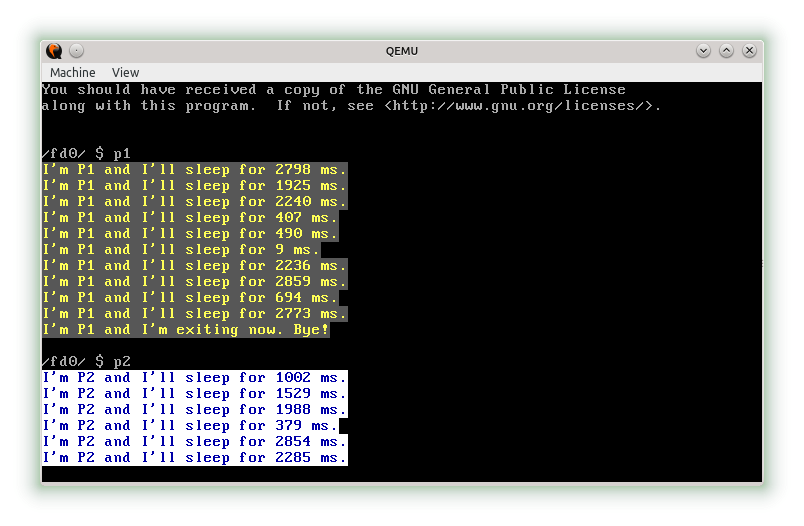
\includegraphics[scale=0.72]{0.png}
    \caption{前台任务}\label{fig:fg}
\end{figure}

\subsection{后台任务}
在控制台中输入程序名称+\&可以在后台运行程序。程序运行后Shell程序将可以继续读取
用户输入的命令。当然,像UNIX的大多数Shell一样,在后台运行的程序的输出将会与
Shell程序的提示符混在一起,但是由于有键盘缓冲区,用户仍然可以继续输入命令。
见图~\ref{fig:bg}。

\begin{figure}[htp!]
    \center
    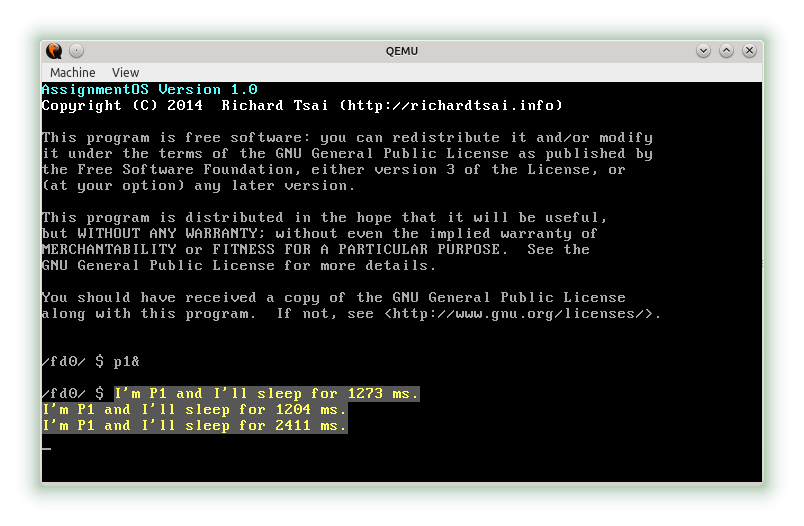
\includegraphics[scale=0.72]{1.png}
    \caption{后台任务}\label{fig:bg}
\end{figure}

\subsection{多任务}
用户可以输入~\verb|p1&|->回车->\verb|p2&|->回车->\verb|p3&|->回车\verb|p4&|回车
(不用管其他进程的输出)同时在后台运行4个程序观察多任务运行效果。全部进程退出
后可以按回车调出命令提示符。见图~\ref{fig:multi}。

\begin{figure}[htp!]
    \center
    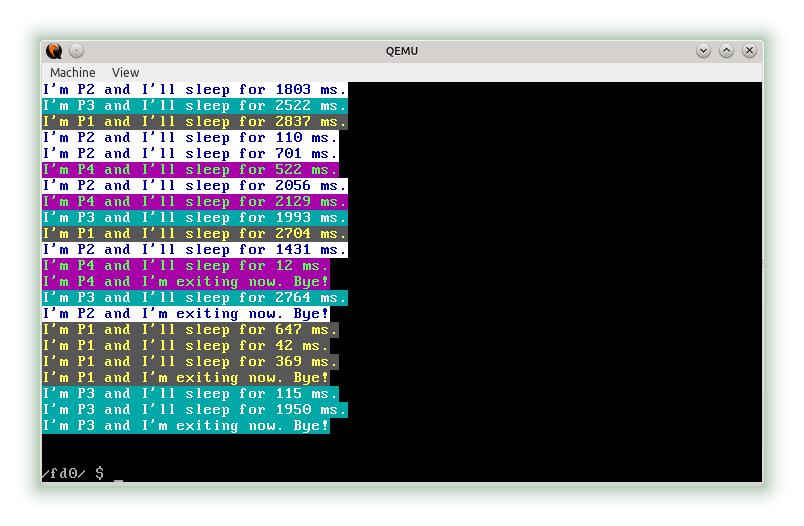
\includegraphics[scale=0.72]{2.png}
    \caption{多任务}\label{fig:multi}
\end{figure}

\end{document}
